%%%%%%%%%%%%%%%%%%%%%%%%%%%%%%%%%%%%%%%%%%%%%%%%%%%%%%%%%%%%%%%%%%%
%                                                                 %
%  GEANT manual in LaTeX form                              %
%                                                                 %
%  Michel Goossens (for translation into LaTeX)                   %
%  Version 1.00                                                   %
%  Last Mod. Jan 24 1991  1300   MG + IB                          %
%                                                                 %
%%%%%%%%%%%%%%%%%%%%%%%%%%%%%%%%%%%%%%%%%%%%%%%%%%%%%%%%%%%%%%%%%%%
\Origin{R.Brun}
\Submitted{01.11.83}        \Revised{16.12.93}
\Version{Geant 3.16}        \Routid{HITS199}
\Makehead{The SET data structure JSET}

\begin{figure}[hbt]
     \centering
     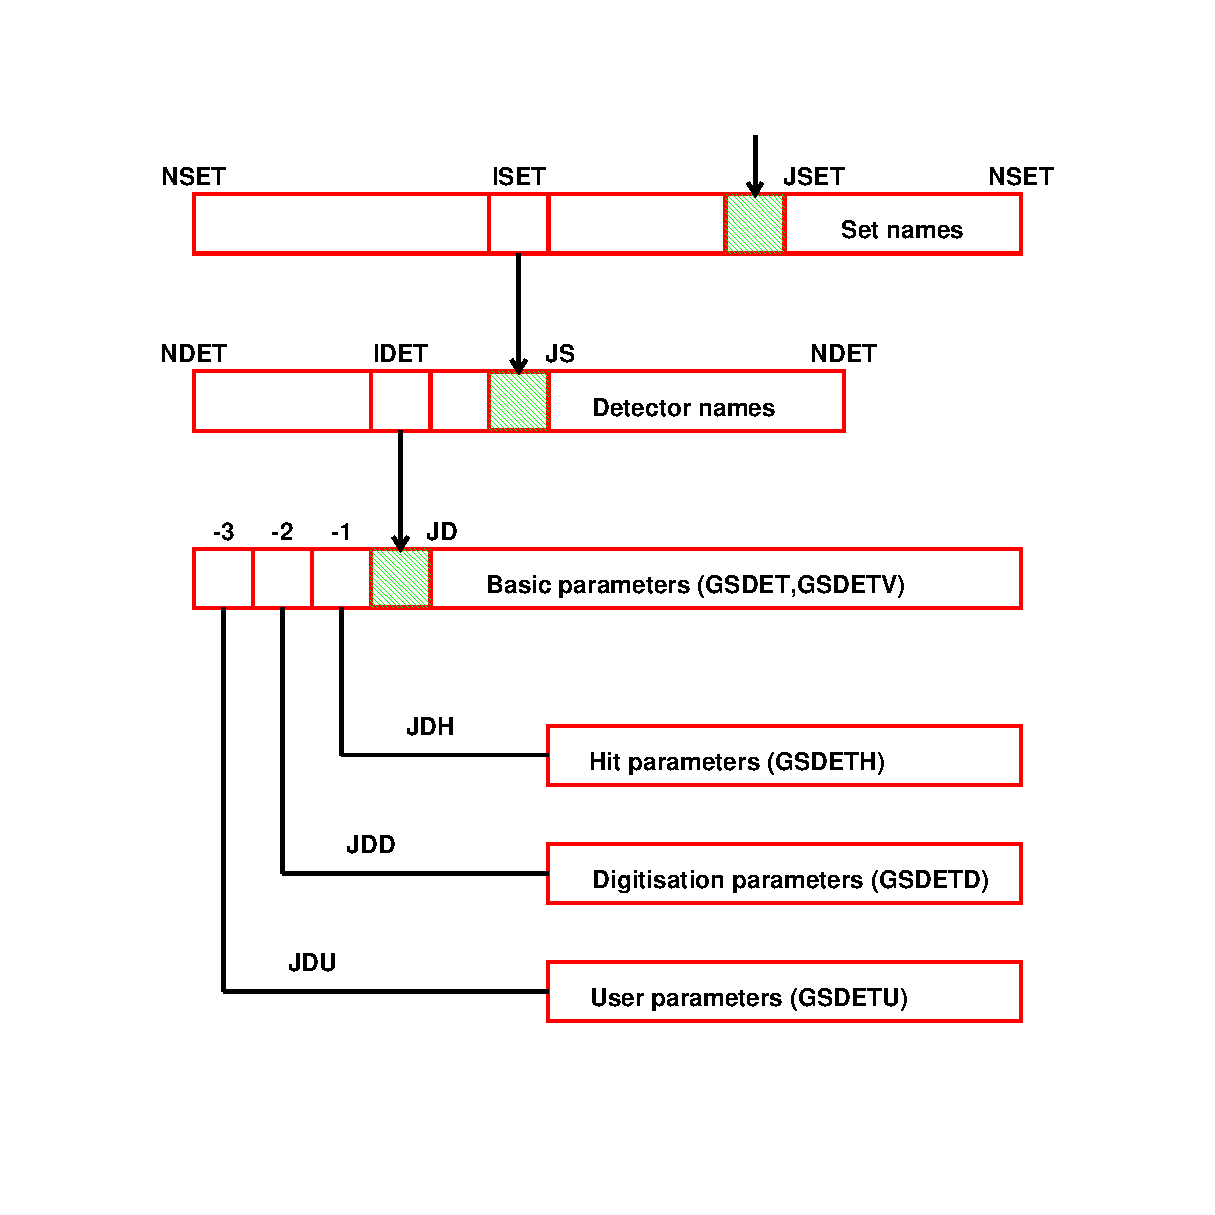
\epsfig{file=eps/hits199-1.eps,width=14cm}
     \caption{Example of geometrical tree structure}
     \label{fg:hits199-1}
\end{figure}
 
{\tt JS} = {\tt LQ(JSET-ISET)} pointer to detector set number {\tt ISET}
The {\tt JSET} data structure is filled by \Rind{GSDET}, 
\Rind{GSDETV}, \Rind{GSDETH}, \Rind{GSDETD}, \Rind{GSDETU} 
and possibly by \Rind{GSDETA}.
 
